%=======================================================================================%
\chapter{Review of the Molecular Cause of Cystic Fibrosis and Its Treatment}
\label{chap:cftr}
\chapquote{Because of what's inside me; Because of my genes.-Bob Flanagan \cite{dick1997}.}{}
\newpage
%Authors note:
% We begin with a breif overview of the disease Cystic Fibrosis as it is the main motiation for this project. A horrendous disease for which we will soon find a cure.

% The purpose of this chapter is to present an overview of CFTR's structure and mechanism of action as discovered by a combination of structural and physiological studies. In addition to the actions of CFTR modulators.

This thesis primarily focusses on the molecular causes of Cystic Fibrosis. In subsequent proceeding chapters we will use Molecular Dynamics (MD) to determine what kind of defect rare mutations cause, with the goal of understanding what kind of treatments they might respond to. Given the imoprtance of the CFTR protein system to the goal of this work we will look at its structure and dynamics in detail in this chapter. However, to understand the motivation for these studies, we will first review some of the medical literature surrounding the disease itself. 

In previous chapters we always worked upward. In chapter \ref{chap:methods} I showed how we can begin from Schr\"oedinger's wave equation to understand biomolecular systems. This was to give an example of the philosophy I outlined in chapter \ref{chap:introduction}, taking abstract formalisms and working upward to model macroscopic biophysical phenomenon. By contrast, I have taken particular care to begin this chapter with a pragmatic discussion of this awful disease. When one trains to practice medicine they are taught a rigorous code of conduct and ethics. I had no such training and I knew I was missing something by studying this disease so impersonally \cite{foucault1994}. I think it's important to note that physicists have had a long history of political and moral philosophy, not always for the better \cite{frank1993, gottfried1999, global2009, rhodes1986, aaronson2008, berger2016, vonneumann_britanica}. Should we wish to embark on the enterprise of studying biophysics we have a responsibility to also study how to do it ethically. These questions have thankfully been studied for some time by philosophers and the reader is referred to texts on bioethics and ethics in artificial intelligence \cite{buchanan2000, genome_editting_guildelines_2017, muller2021, bostrom2014}. As biophysical techniques increase capability, so does their capability for misuse \cite{mallapaty2022, urbina2022}. 

%On this somewhat somber note, we will now take a brief look at what it is like to live with Cystic Fibrosis.

%We will then analyse the root cause, mutations to the Cystic Fibrosis transmembrane Conductance Regulator (CFTR). In chapter \ref{chap:conclusion} we will use much of the knowledge gained in this chapter to think about where we can direct future studies to help treat the root cause of Cystic Fibrosis. 


\section{Clinical outcomes of Cystic Fibrosis}
Cystic Fibrosis (CF) is the most common fatal genetic condition in Caucasian populations. 165 000 people are estimated to be afflicted globally \cite{guo2022}. Even with decades of research there is no known cure for CF. With the average life expectancy of patients falling below 50 even in countries with developed health care systems such as the USA and Australia\cite{mcbennett2022}. The symptoms of the disease are due to the inability of cells to regulate their salt content. 

The most acute symptoms are due to the dehydration of epithelial membranes. When dehydrated the cilia on the epithelium collapse leaving them unable to clear the mucus that naturally lines the airway\cite{boucher2007}. The dehydration mentioned earlier causes the mucus to thicken. This buildup has two pathogenic functions. Firstly it inhibits the normal function of the organ, as mucus fills ducts that would normally pass nutrients in the pancreas or absorb gasses in the lungs. Secondly, the stationary mucus allows bacterial infection, this can further degrade lung function and remains one of the most troublesome chronic complications in CF patients. 

Much of the clinical research into CF has been managing the movement of this mucus and the populations of bacterium in it. Patients require hours of physical therapy each day to help clear this mucus since their lungs are unable to. They must also inhale saline solutions in order to counteract the osmotic pressure in their epithelium. This helps draw more moisture out of the epithelial cells to allow the cilia to move. 

CF patients struggle to intake nutrients due to the build up of mucus in the ducts of their pancreas and large intestines. This leads to CF related diabetes which afflicts roughly half of adults with CF \cite{Kayani2018}. Patients with CF related diabetes are often administered enzymes and must adhere to a specific diet. 

\begin{figure}
	\label{CF_life_expectancy}
	\begin{center}
	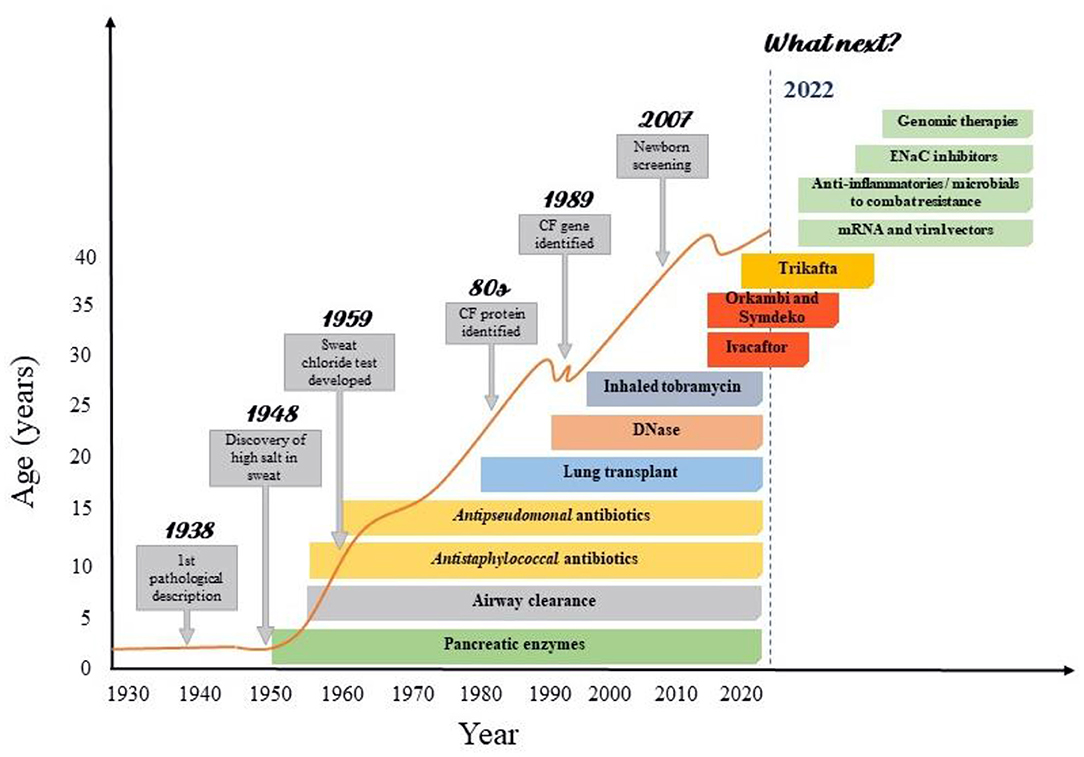
\includegraphics[width=0.6\textwidth]{figures/CF_life_expectancy.png}
	\end{center}
	\captionsetup{singlelinecheck = false, justification=raggedright}
	\caption[CF Clinical Progress] {\textbf{CF Clinical Progress}}{Life expectancy of CF patients correlates highly with translational research. Source \cite{garcia2022}} 
\end{figure}

These complicated clinical factors have lead to an array of treatments to manage the disease. Patients must undergo hours of physical therapy each day in order to aid in the clearance of mucus from their lungs, they must adhedre to a specific diet . What is remarkable is that modulators have been shown to aid in the releif of these symptoms \cite{lopes-pacheco2020}.

\section{CFTR Structure}

\begin{figure}
	\begin{center}
	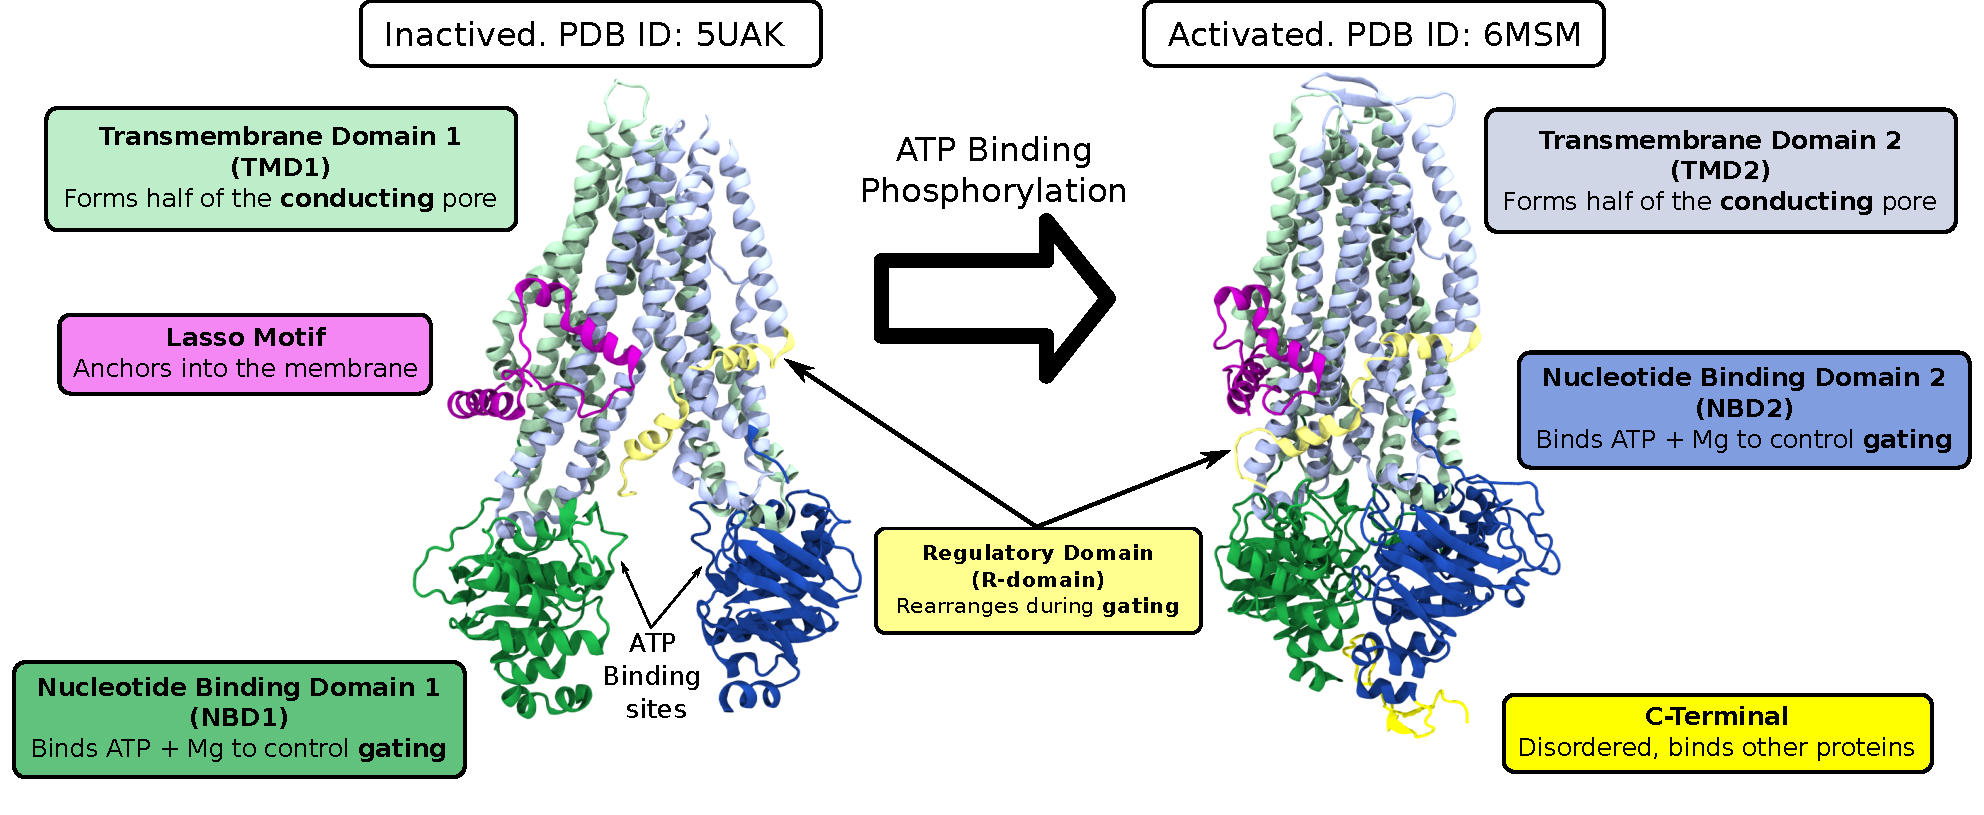
\includegraphics[width=\textwidth]{figures/CFTR_structure.pdf}
	\end{center}
	\label{CFTR_structure_domains}
	\captionsetup{singlelinecheck = false, justification=raggedright}
	\caption[CFTR Structure] {\textbf{CFTR Structure}}{There are currently two resolved human structures. The inactivated state is neither phosphorylated nor bound to ATP. Observe how the NBDs are far apart and the TMDs are not parallel, forcing a constriction which does not allow the passage of ions. By contrast, the activated structure is abound to ATP at both sites, bringing the TMDs into a parallel configuration where they form a pore. There are unresolved questions as to whether CFTR may conduct chloride in this conformation which we will analyse in chapter \ref{chap:opening}.} 
\end{figure}
CFTR is composed of one chain with pseudo-symmetric structure, the protein is well organised into 7 domains \ref{CFTR_structure_domains}. In the order of their primary structure they are: 
\begin{enumerate}
	\item The Lasso motif (AA 1-68). Anchors into the membrane and serves as an interaction hub with protein partners such as syntaxin and filamin which are important in cellular trafficking \cite{cormet-boyaka2002, naren1998, thelin2007} as well as WNK1 which plays a role in bicarbonate selectivity \cite{kim2019}.
	\item Transmembrane Domain 1 (TMD1 AA 69-376). This domain forms half of the chloride conducting pore and importantly, TM1 and TM6 in this domain form the extracellular end of the pore for anion permeation \cite{linsdell2006, linsdell2022}.
	\item Nucleotide Binding Domain 1 (NBD1 AA 377-629). One of the ATP binding sites, this domain has a dense concentration of disease causing mutations, including the most common mutation $\Delta F508$ \cite{cftr2}.
	\item Regulatory Domain (R-domain AA 630-855). A disordered domain containing up to 11 phosphorylation sites\cite{mihalyi2020}. In the inactivated conformation a helical segment of this domain wedges between the TMDs. Upon binding of PKA and phosphorylation the wedge relocates to a location just below the R-domain. The identity of a fragment of the R-domain is analysed in detail in chapter \ref{chap:I37R}. The kinetics of this domain is important to the overall function of CFTR \cite{ostedgaard2000, mihalyi2020}. 
	\item Transmembrane Domain 2 (TMD2 AA 856-1168). This domain forms the other half of the chloride conducting pore. There is ongoing controversy over the structure and function of TM8 the function of CFTR \cite{hegedus2022, liu2019}.
	\item Nucleotide Binding Domain 2 (NBD2 AA 1169 - 1450). Home to the conserved Q-loop, which plays an important role in the binding of ATP in ABC transporters \cite{ivey2020, zolnerciks2014, dong2015}.
	\item C-terminus (NBD2 AA 1451 - 1480). This structure is natively disordered but it serves as an interaction hub in WT-CFTR, anchoring CFTR to other proteins through its PDZ binding domain \cite{moyer1999, cushing2008}. 
\end{enumerate}
Transmembrane Domain 1 (TMD1) which forms half of the pore. Nucleotide Binding Domain 1 (NBD1) which binds ATP when the channel is in the open state. The Regulatory domain (R-domain) which, when phosphorylated allows the channel to open. Transmembrane domain 2 (TMD2) which forms the other half of the ion conducting pore. Nucleotide Binding Domain 2 

CFTR belongs to a super family of proteins known as ATP Binding Cassette Transporters,  many of these proteins perform active transport across cell membranes. The substrates they transport can vary, including lipids and drug molecules. Proteins in this family share a common motif known as Nucleotide Binding Domains (NBDs). These domains act as ATPases, accelerating the hydrolysis of ATP. The energy from hydrolysis is then transferred into the protein in order for it to pump its substrate against a concentration gradient. 

\section{CFTR is a Unique ABC Transporter}

\begin{figure}
	\label{ABC_diversity}
	\begin{center}
	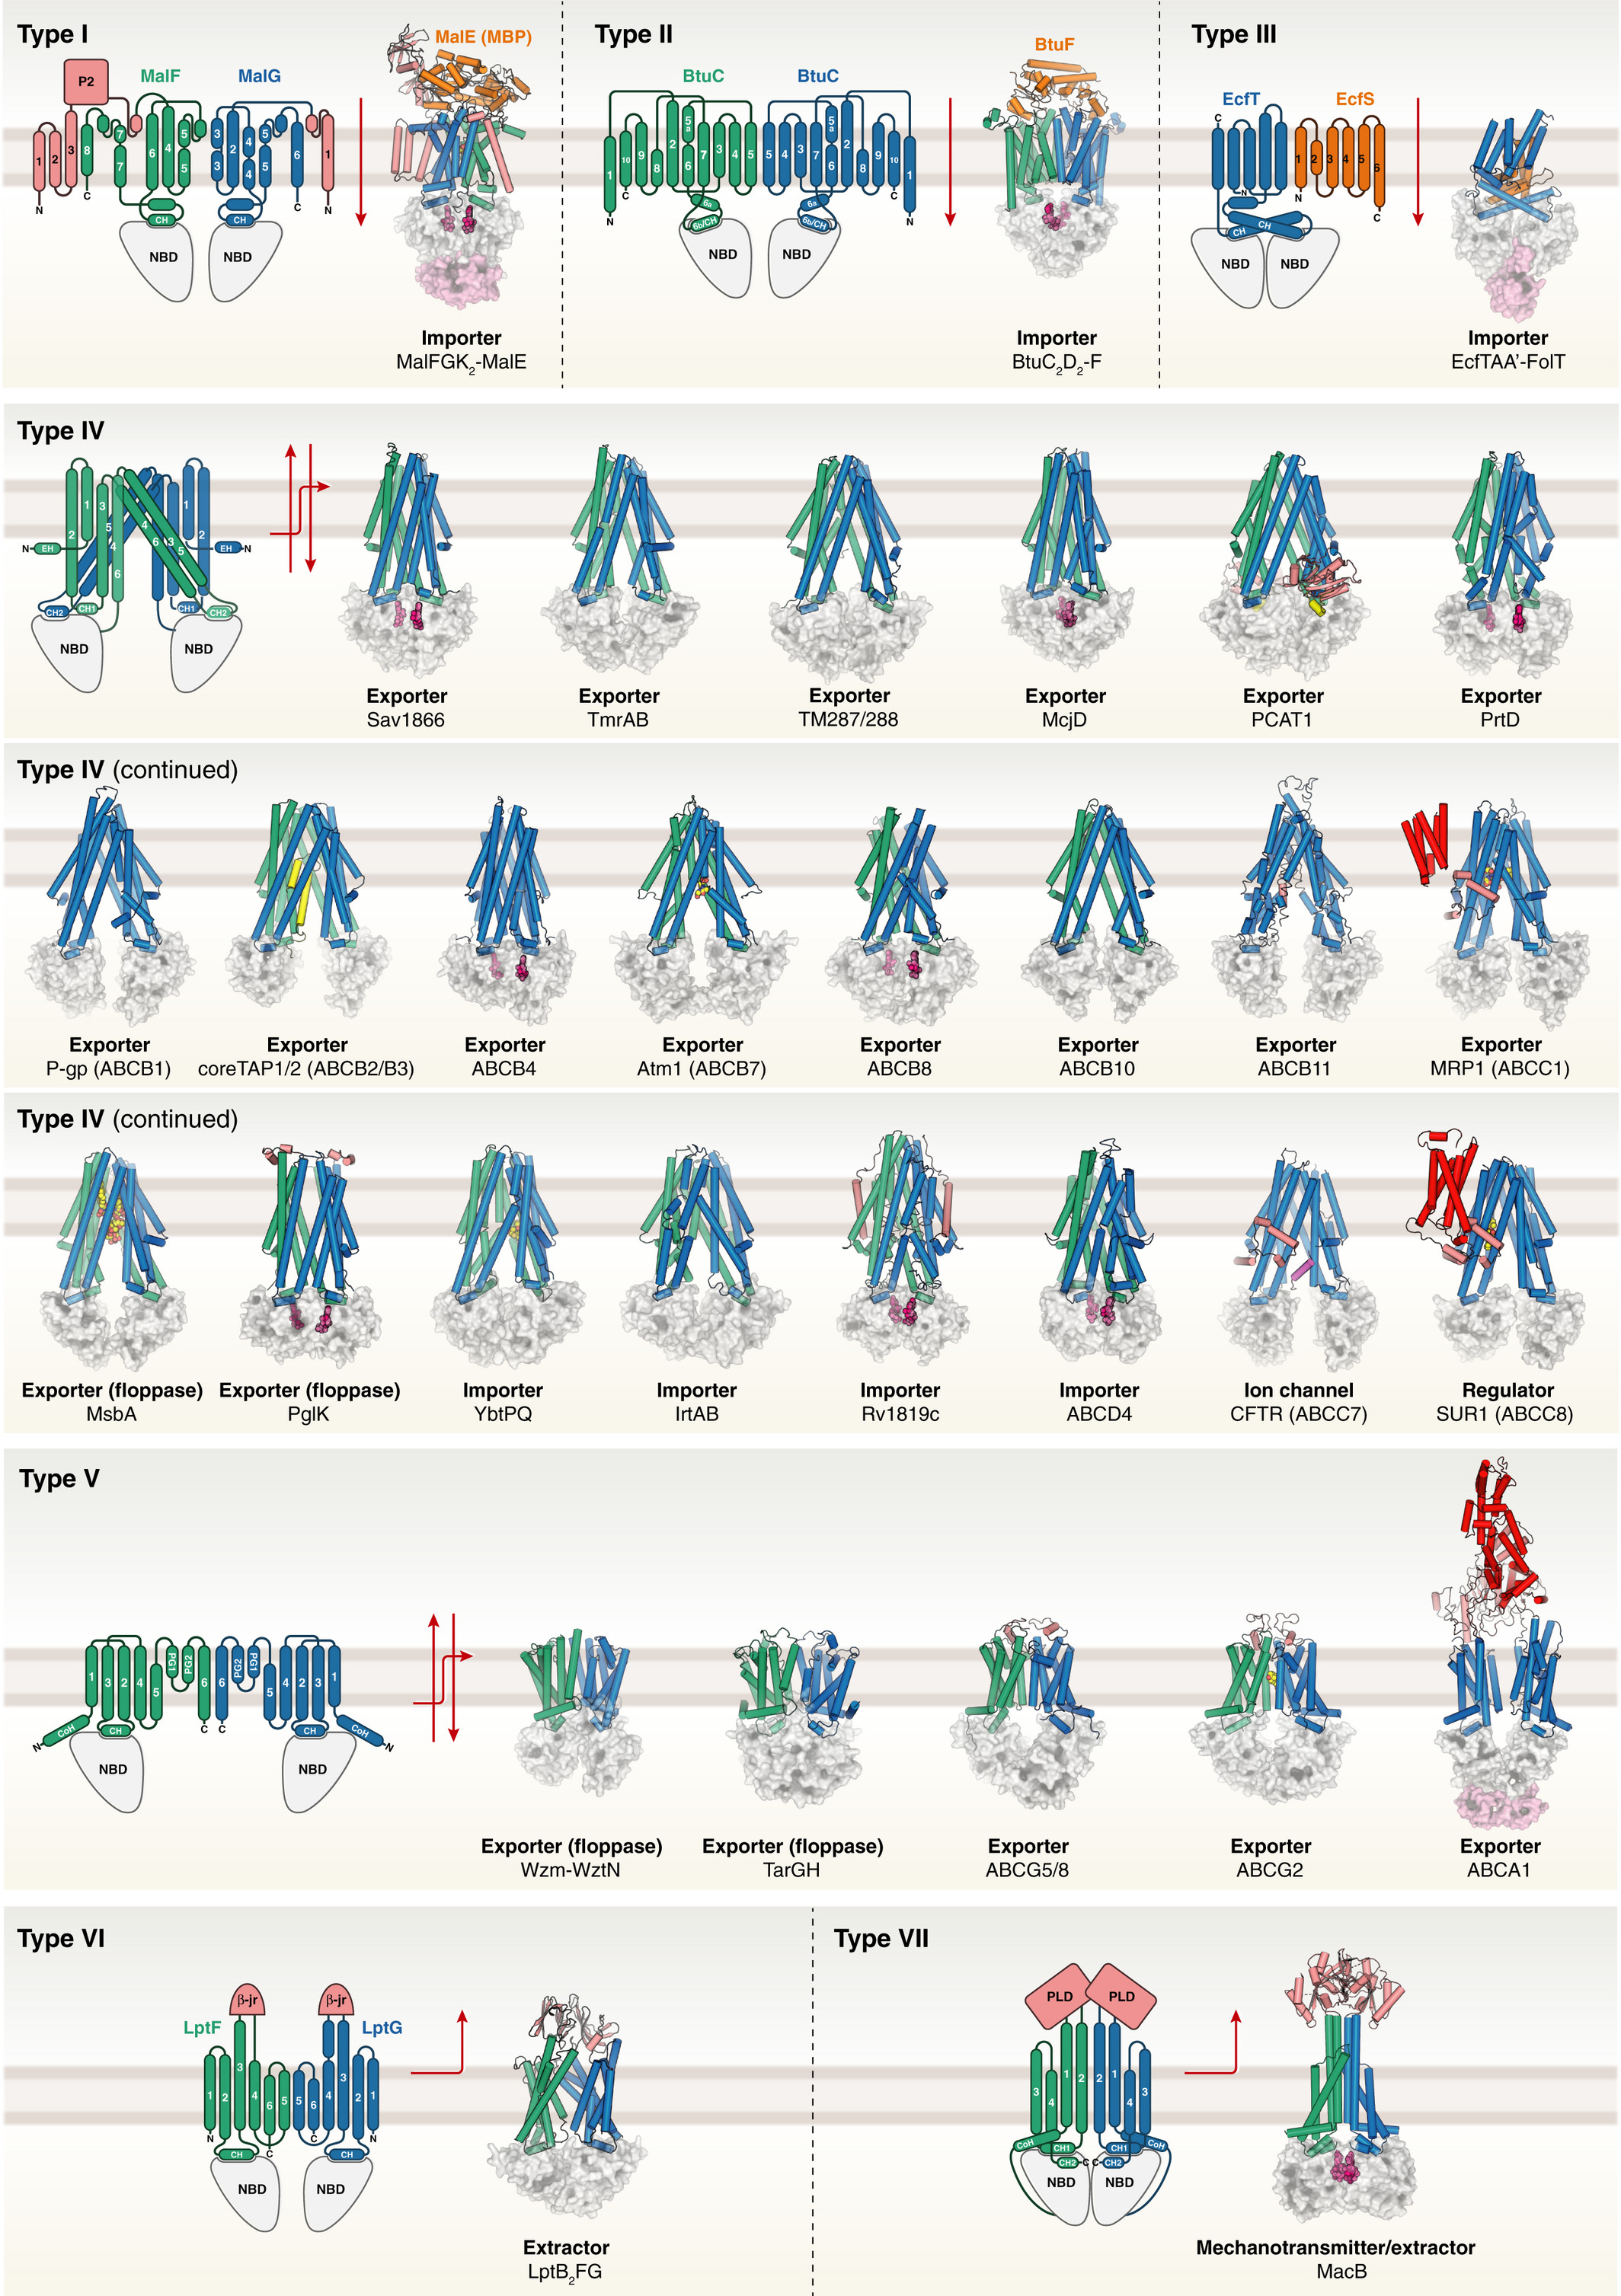
\includegraphics[width=\textwidth]{figures/ABC_classification.jpg}
	\end{center}
	\captionsetup{singlelinecheck = false, justification=raggedright}
	\caption[CFTR Structure] {\textbf{CFTR Structure}}{The structural diversity of ABC transporters. Structures are classified based on the organisation of their TMDs source \cite{thomas2020}.} 
\end{figure}
ATP-Binding Cassette (ABC) transporters are an intriguing super family of proteins. On the whole, they transport substrates by using a combination of phosphorylation energy from ATP hydrolysis. These can be diverse substrates such as lipids or small molecules. Their structural diversity can be seen in figure \ref{ABC_diversity} reflecting their array of functions. 

CFTR is unique, as it is not a transporter, but rather an anion \textit{channel}. The kinetic energy of the ATP is not used to translocate substrate across the membrane but rather simply used in the regulation of the gating cycle. Chloride, bicarbonate and other anions are able to \textit{passively} diffuse through the channel. This evolutionary misappropriation of a transporter to a "leaky channel" is perhaps the reason so many mutations can create a non-functional protein \cite{linsdell2018}.

\section{The Misfunction of CFTR causes CF}

The primary cause of the disease Cystic Fibrosis (CF) is the malfunction of a chloride channel, the Cystic Fibrosis Transmembrane Conductance Regulator (CFTR). This ion channel is a member of the ABCC subfamily of ABC transporters, designated ABCC7. This channel is unique amongst this family because it is not generally considered an active transporter but something of a low conductivity channel or a "weak pump"\cite{linsdell2018}.

CFTR is distinguished by a regulatory region known as the R-domain (residues 645-845) which links NBD1 to TMD2. This region acts to lock the channel in the closed state by wedging itself between the TMDs and dislodging when any one of 3 sites are phosphorylated \cite{mihalyi2020}. In experimentally determined structures of human CFTR the secondary structure of a section of the R-domain but not at high enough resolution to determine the identity of individual side chains \cite{zhang2018, zhang2016}. Further secondary structure information can be found through experiments with NMR \cite{Baker2007}.

Previous computational studies of CFTR have been used homology models based on the phosphorylated zebra fish protein PDBID:5W81 \cite{zhang2017a}. These have yielded interesting results but the sequence similarity between human and zebra fish CFTR is only 55\% \cite{}. For a protein structure where a single amino acid mutation leads to malfunction, more precision can only help. Additionally, the activity of CFTR modulators is not conserved in mutant zCFTR possibly because it has different kinetics to the human channel \cite{}. In order to do precision medicine we need precision structures. 

An open state of the channel has been proposed by combining both the zebra fish homology model and the fully outward facing conformer of a bacterial ABC transporter Sav1866 \cite{Hoffmann2018}. Although this model has several characteristics expected of the open channel, such as the critical R352-D993 salt bridge, it lacks a salt bridge between R104-E116. In experiments, these residues could be replaced by cysteines and the channel would still function. However, when reducing agents were added to the system the channel lost its ability to open fully. This indicates that in the oxidised environment the C104-C116 cysteines formed a disulfide bridge but its breaking upon exposure to reducing agents caused a loss of function in the channel. This indicates that in the WT channel R104-E116 form a stable salt bridge. 

This salt bridge is clearly visible in the recent cryo-EM structure of ATP-bound human CFTR \cite{zhang2018}.

\subsection{The Gating Cycle}
The conformational transition from inactive to active differs significantly in CFTR compared to other ABC transporters. The NBDs are largely similar to other to those found in other ABC transporters, they dimerise in what is termed a head to tail configuration so both subunits contact both bound ATP molecules \cite{} See FIGURE. Residue E1371 allows nucleophilic attack by surrounding water on the $\gamma$ phosphate  of the ATP bound to Walker B \cite{Stratford2007}. The hydrolysis of ATP is the event which causes the channel to gate back to the closed conformation \cite{}. 

\subsection {Anion Selectivity}
CFTR is weakly selective for specific anions. F337 is the most important amino acid for selectivity. Bicarbonate (HCO$_3^-$ is known to have roughly 26\% the permeability of chloride through the channel. Note that Fluoride has even higher conductance through CFTR, likely due to its small size and high solvation energy (does this indicate hydrated conductance?). WNK1 is known to influence the selectivity of the channel https://www.ncbi.nlm.nih.gov/pmc/articles/PMC6889609/. The permeation of bicarbonate is very important physiologically because if a mutation permeates bicarbonate it means there is a high likelihood the patient will be pancreatic sufficient. 

Compared to cation channels like Gramicidin and KcsA, CFTR is only weakly selective, permeating a large set of anions with varying radii and geometries. Supposedly it is more permeant to lyotropic (low solvation energy anions) rather than cosmotropic anions (high solvation energy anions) indicating that dehydration of the anion is likely during conductance (CITATION NEEDED). The radius of hydrated chloride ions is 1.7A\cite{yang2002} so even with this larger pore partial dehydration must take place. 


\section{Classes of Mutation Which Cause Cystic Fibrosis}
The 360 disease causing mutations to CFTR have been classified into 6 common classes based on the nature of the CF they cause, their reaction to CFTR modulators, and results \textit{in vitro} assays. Ultimately I aim to show that at the atomic level these classes of mutations are less meaningful and as patient specific theratyping evolves these classes will become less relevant, serving as illustrative tools only to communicate at a higher level what is going wrong with the CFTR protein. The canonical classification is as follows:
\begin{itemize}
	\item \textbf{Class I} No functional protein. Under these mutations no protein is transcribed due to either problems with the transcription of mRNA or a premature stop codon truncating protein synthesis early, meaning the resulting peptide is missing key domains. 
	\item \textbf{Class II} Folding defect. These mutations cause the translated peptide to misfold into the incorrect tertiary structure. This can inhibit the protein's journey as it is trafficked to the cell membrane, its function while once it is there or its functional life time at the surface. 
	\item \textbf{Class III} Impaired Gating. Here the mutation inhibits the ability of the protein to transition from the closed to the open state. 
	\item \textbf{Class IV} Decreased Conductance. These mutations cause a barrier in the energy landscape of the CFTR chloride conductance pathway.
	\item \textbf{Class V} Less Protein Expressed.  
	\item \textbf{Class VI} Decreased Lifetime

\end{itemize}

Although useful, in reality this paradigm struggles to reflect the fact that a mutation can belong to multiple categories to different levels due to different modes of pathogenesis. Through our molecular simulations we can see that in reality CFTR modulators are capable of treating several different mutations with very different molecular fingerprints. We will break down this paradigm into more molecular detail in chapter \ref{chap:outlook_review}

FIGURE demonstrates how each of the canonical classes at the molecular level is broken down into many sub classes and a mutation might belong to one of many of these subclasses. Structural biology paradigms and \textit{in silico} modelling can help classify mutations into these different classes. In combination with wet lab assays we can understand which classes of these molecular defects are most effectively treated with specific drug regimens. Our computational microscope is helping choose treatments for patients at the atomic level. 

\section{CFTR Modulators}
Since CF is caused by malfunctions of the channel it makes sense to pursue CFTR as a drug target. Through high throughput \textit{in vitro} screening several (GET NUMBER) compounds have been developed that aim to rescue the function of CFTR. These fall into two classes. Correctors, which aid CFTR to fold into the correct state and potentiators which help the channel reach the fully open state once it has already folded correctly. Emerging evidence suggests that specific genetic defects may be optimally rescued by specific combinations and doses of both correctors and potentiators compounds. Recently, cryo-EM structures of these compounds in their bound state have been released. In addition to several \textit {in vitro} biophysical experiments to determine the precise mechanism of action and binding site of these compounds.

\subsection{Correctors}
The mechanism of action for corrector compounds appears to be to bind to to a pocket between TMH1 and TMH3. Circular dichromism and fluorescence experiments found that an isolated construct of TMH3 and TMH4 were more likely to fold correctly in the presence of corrector compounds. Later cryo-EM structures discovered high resolution electron density in the pocket in the shape of the drug compounds \cite{fiedorczuk2022}. 

In combination this is strong evidence for the precise mechanism of action for corrector compounds. Further work will aid in the creation of new compounds to refine our exploitation of this mechanism.

\subsection{Potentiators}
There is more uncertainty surrounding the mechanism of potentiators drugs. Experiments clearly demonstrate that they act directly on CFTR in order to increase the likelihood that it occupies the open state. They bind to the protein with picomolar affinity. There are are cryo-EM structures which show the drugs bound to the TM8 hinge region \cite{}. \textit {In vitro} experiments suggest at least two membrane facing binding pockets due to the drugs extreme hydrophobicity\cite{}. The location of this second binding site is unknown. The difficulties arise with mutagenesis experiments. The dose-response curves in several studies show that when various sites are mutated the activity of the drug is lowered. This indicates additional binding sites not yet well defined. 

GLPG1837 has not been approved in a clinical setting. \textit {In vitro} experiments suggest that it is more efficacious even though it has lower affinity for CFTR binding (CITATION NEEDED). This would indicate that the highest affinity binding pocket does not produce the greatest modulation. More work is needed to resolve the mechanism which results in the clinical effectiveness of these drugs.  

These drugs are clinically efficacious \cite{VanGoor2014} on several mutants with some curious exceptions like N1303K. I suggest the following mechanism for their action. I suspect a similar analogy exists for the action of the correctors. WT-CFTR exhibits a natural landscape with kinetic barriers in the transition between the closed and open states. A gating class mutation to CFTR will introduce a kinetic barrier in the pathway of this conformational transition. What these drugs do is reduce a barrier in the existing conformational landscape of CFTR. This compensates for the barriers introduced by the mutation. 

This provides a rationale for why it appears possible for diverse range of molecular defects to be treatable by these small molecules. In our work we've found that the atomic nature of the defects introduced by each mutation varies widely, what is interesting is that experiments in \textit{ex vivo} models have shown that these drugs treat a variety of different defects. The classification of classes of defect is outdated, really there are as many classes as there are mutations.


\subsection{Patients with rare mutations struggle to gain access to modulator therapy}

\section{Patient Derived Organoids as a Pre Clinical Model}
The basic unit of living things are cells. In the medical field there is growing capability to discern the functioning of an individual patient's cells. These can be used as models for testing what might produce the best clinical outcomes for the patient. For the case of Cystic Fibrosis researchers have begun to take samples of epithelial stem cells of patients with the disease and grow those samples into tissues which mimic the function of the entire organ\cite{depoel2020}. This is possible in the epithelium due to a population of adult stem cells which maintain the ability to differentiate into a variety of cell types (a property known as pluripotency). 

Primarily, these epithelial stem cells are taken from the nasal passages of patients or from rectal biopsies. These samples can then be grown into organoid models of the lung or gut respectively. 

Adult stem cells in the epithelium are preferable because other sources of stem cells such as induced pluripotent stem cells (iPSCs) require complex, time consuming protocols to grow into fully developed organoids. Already the differentiation and expansion of epithelial samples takes a month \cite{}.

In the case of CF this technology allows the construction of a scalable, patient specific platform where a patient's own tissues can be tested to determine the best treatment for them. These pre-clinical models will allow more patients in the heterogeneous set of disease causing mutations to access modulators. This has given rise to an exciting prospect of a practice known as theratyping, enabling clinicians to make a personalised choice of which drugs which drug regimen will best serve a patient \cite{clancy2019, wong2022, wong2022a, ciciriello2022}. This thesis demosntrates that integration of \textit{in silico} simulations into this process can further the capabilities of these pre-clinical models.

%One limitation of these organoid platforms is the lack of an inflammatory response since no immune cells are present in the tissue culture. 
The response of the patient's epithelium is characterised using a few \textit{in vitro} assays which we will briefly discuss below. 

\subsection{Forskolin Induced Swelling}
Forskolin Induced Swelling (FIS) assays have been used to characterise the patient specific response of a patient's organoids to a drug regimen \cite{dekkers2013}. When epithelial cells are exposed to a chemical known as Forskolin they begin to rapidly produce cyclic AMP (cAMP, a precursor to ATP in a cell) \cite{}. This allows the down stream activation of CFTR ion channels, causing the organoids themselves to swell. This swelling allows cell biologists to easily quantify the activity of CFTR within a patient, in a variety of conditions.

\subsection{Cilia Beating Frequency}
The lungs are covered in cilia which fluctuate or "beat" in order to clear mucus and other particles in the respiratory tract \cite{mitchison2010, bustamante-marin2017}. One of the most characteristic symptoms of patients with Cystic Fibrosis is the build up of mucus around the epithelium. This causes cilia to collapse, meaning they cannot move \cite{}. By measuring .

\subsection{Electrophysiology}
Since CFTR is an ion channel, measuring its electrical activity is a direct way to assess its function. For single channel studies this is done with a patch clamp. However, this does not give an assessment of the whole epithelium. Often the whole organoid is used as a patch and put in an Ussing chamber. By blocking other ion channels such as ENAC a clear picture of CFTR function can be measured in order to create a pre-clinical model for a specific patient.

\subsection{Western Blotting to Assess CFTR Trafficking}
The above methods may be able to properly quantify gating class mutations but they will struggle to assess the amount of CFTR at the cell surface. For this we employ .
